\section{Versuchsdurchf�hrung und Auswertung}
%erkl�ren, !was! wir machen, !warum! wir das machen und mit welchem ziel
%(wichtig) pr�zize erkl�ren, wie bei dem versuch vorgegangen und was gemacht wurde
%\subsection{Verwendete Formeln}
%eine legende kann angefertigt werden, die selbstverst�ndlichen buchstaben m�ssen nicht extra erkl�rt werden
%mit knappen erkl�rungen die !verwendeten! formeln, sowie die zugeh�rige fehlerrechnung einf�gen.
%\subsection{Messergebnisse}
%die messwerte in !�bersichtlichen! tabellen angegeben
%zu viele kleine tabellen in gro�e tabellen �berf�hren!
%zu gro�e tabellen mit dem [scale]-befehl scalieren oder (falls zu lang) in zwei kleinere tabellen aufteilen
%(wichtig) vor !jeder! tabelle sagen, was gemessen wurde und wie die fehler gew�hlt wurden und ausreichend !erkl�ren!, !warum! wir unsere fehler grade so gew�hlt haben
%\subsection{Auswertung}
%zuerst !alle! errechneten werte entweder in ganzen s�tzen aufz�hlen, oder in tabellen (�bersichtlicher) dargestellen, sowie auf die verwendeten formeln verweisen (die referenzierung der formel kann in der �berschrift stehen)
%kurz erw�hnen (vor der tabelle), warum wir das ganze ausrechnen bzw. was wir dort ausrechnen
%danach histogramme und plots erstellen, wobei wenn m�glich funktionen durch die plots gelegt werden (zur not k�nnen auch splines benutzt werden, was aber angegeben werden muss)
%bei fits immer die funktion und das reduzierte chiquadrat mit angegeben, wobei auf verst�ndlichkeit beim entziffern der zehnerpotenzen geachtet werden muss z.b. f(x)=(wert+-fehler)\cdot10^{irgendeine zahl}\cdot x + (wert+-fehler)\cdot10^{irgendeine zahl}
%bei jedem fit erkl�ren, nach welchem zusammenhang gefittet wurde und warum!
%bei plots darauf achten, dass die achsenbeschriftung (auch die tics) die richtige gr��e haben und die legende im plot nicht die messwerte verdeckt
%kurz die aufgabenstellung abhandeln 
Die mittlere Flachen- bzw. Linien-Rauheit (CC-Mode), die Gitterstruktur, die Atomabst�nde und im glatten Bereich die Elektronendichteverteilung von [HOPG]-Graphit (CH-Mode) soll aus den mit dem RTM gemessenen Daten bestimmt werden. Danach soll die Fl�chen- und Linien-Rauheit, monoatomare Stufen, Gitterfehler und Stufenh�hen, sowie Gitterparameter einer (111)-Goldschicht (CC-Mode) erfasst werden. Zuletzt soll eine unbekannte Probe mit geeigneten Messungen untersucht werden.
\subsection{Graphit}
Die Graphitschicht konnte magnetisch auf der Probenhalterung angebracht werden. Die Vorbereitungen f�r die Graphitmessung dauerten nicht lange, da nach wenigen Versuchen eine funktionsf�hige Pt-Ir-Spitze angefertigt werden konnte. F�r die Anfertigung der Pt-Ir-Spitze standen Isopropanol, Reinigungst�cher, eine Pinzette und geeignete Zangen zum anspitzen und halten des Pt-Ir-Drahtes zu Verf�gung.
\subsubsection{Rauheit}

\subsubsection{Gitterstruktur und Elektronendichteverteilung}
\subsubsection{Mittlerer Atomabstand}
\subsection{(111)-Goldschicht}
Die Rauheit der Goldschicht sollte mit dem RTM bestimmt werden. Dazu wurde die Oberfl�che der Goldschicht mit dem RTM im CC-Mode abgerastert.
Wegen der Kornstruktur wurden f�r die Bestimmung der Fl�chenrauheit zwei Messungen vorgenommen, sodass Korngrenzen nur in der ersten Messung in die Berechnung der Rauheit eingingen. Die (111)-Goldschicht musste aufgrund von Kratzern auf der Oberfl�che mehrfach gedreht werden. W�hrend der Justierung ist die Pt-Ir-Spitze des RTM mit der Oberfl�che der Goldschicht kollidiert, sodass eine zweite Pt-Ir-Spitze angefertigt werden musste. Diese konnte ebenfalls nach wenigen Versuchen aus bereits benutzten Pt-Ir-Spitzen angefertigt werden. Zu erste wird eine Aufnahme mit maximalem Scanbereich gemacht, dabei wird die tip-Voltage von 50mV auf 500mV erh�ht, um ein sch�rferes Bild zu erhalten. In Abbildung \ref{fig:gold_maximal_scan} ist die Aufnahme mit maximalem Scanbereich zu sehen.

\begin{figure}[H]
	\centering
  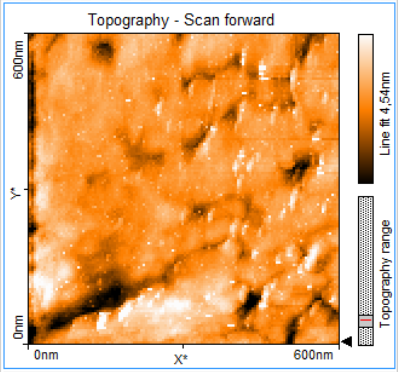
\includegraphics[scale=0.6]{gold_600nm_topographie_oberflaeche.png}
	\caption{Aufnahme der Gold(111)-Schicht mit einer tip-Voltage von 500mV. Im rechten Bereich der Abbildung ist die Kronstruktur der Probe gut zu erkennen.}
	\label{fig:gold_maximal_scan}
\end{figure}

In Abbildung \ref{fig:gold_maximal_scan} ist vor allem im rechten Bereich die  Kornstruktur des Goldes zu sehen. F�r die Aufnahme wurden die Verkippungen bereits korrigiert.

\subsubsection{Rauheit}
F�r die Untersuchung der Oberfl�chen- und Linien Rauheit wurde ein Bereich von 202nm ausgew�hlt. Da ein m�glichst glatter Bereich gew�hlt werden sollte, wurde der obere linke Bereich in aus Abbildung \ref{fig:gold_maximal_scan} ausgew�hlt. In Abbildung \ref{fig:gold_linie} ist eine Aufnahme des Bereichs zu sehen.


\begin{figure}[H]
\centering
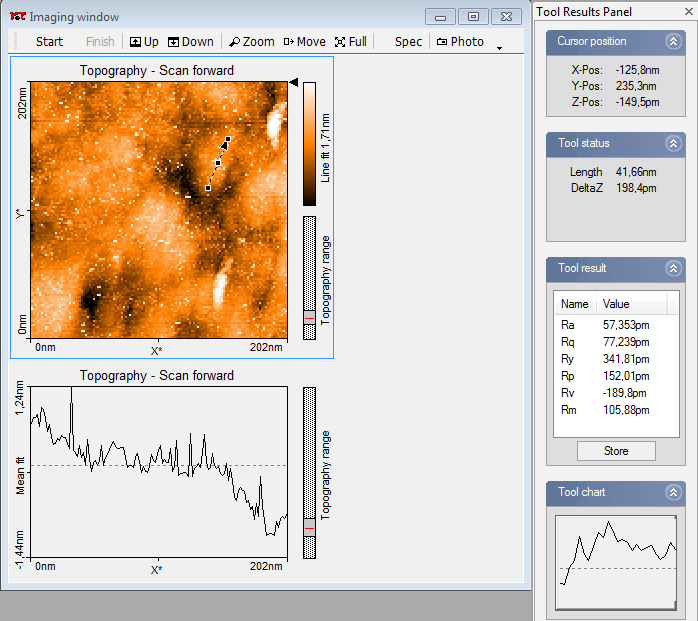
\includegraphics[scale = 0.75]{Gold_linienrauheit_202nm}
\caption{ Mittlere Linienrauheit der (111)-Goldschicht ($R_a = \SI{57,353}{pm}$ und $R_q = \SI{77,239}{pm}$) }
\label{fig:gold_linie}
\end{figure}

\begin{figure}[H]
\begin{subfigure}[t]{0.49\textwidth}
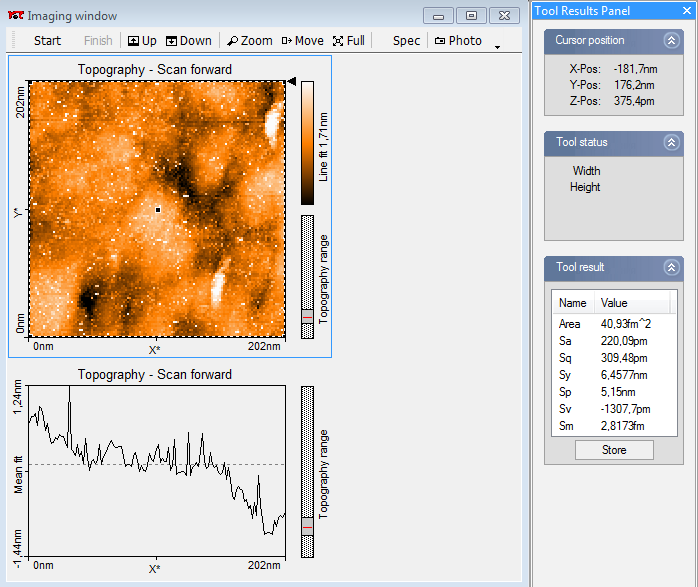
\includegraphics[scale = 0.45]{Gold_flaechenrauheit_202nm_2}
\caption{Mittelung �ber die gesamte Fl�che, da durch die Kornstruktur keine gro�e glatte Fl�che zu finden war. ($S_a = \SI{220,09}{pm}$ und $S_q = \SI{309,48}{pm}$)}
\label{subfig:gold_oberflaeche_1}
\end{subfigure}
\hspace{0.02\textwidth}
\begin{subfigure}[t]{0.49\textwidth}
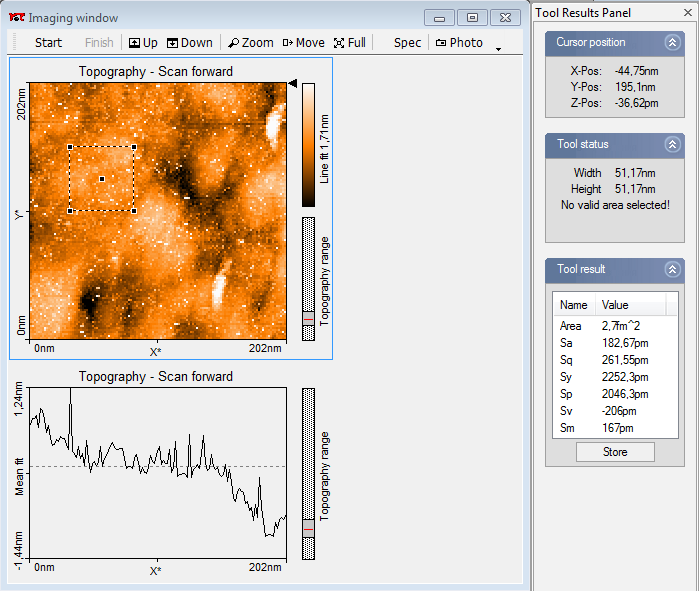
\includegraphics[scale = 0.45]{Gold_flaechenrauheit_202nm_1}
\caption{Mittelung eine kleinere m�glichst glatte Fl�che. Die Verkippung wurde bei allen Messungen korrigiert. ($S_a = \SI{182,67}{pm}$ und $S_q = \SI{261,55}{pm}$)}
\label{subfig:gold_oberflaeche_2}
\end{subfigure}
\caption{ Mittlere Fl�chenrauheit der (111)-Goldschicht}
\label{fig:rauheit}
\end{figure}



Die Oberfl�chenrauheit wird f�r die gesamte Oberfl�che und f�r die glatte Oberfl�che oben links bestimmt (vgl. Abbildung \ref{subfig:gold_oberflaeche_2}). Bei der Bestimmung der Oberfl�chenrauheit, wurden die Werte in Tabelle \ref{tab:rauheit_gold} bestimmt, daf�r wurde die Funktion von easy2Scan verwendet.

\begin{table}[H]
\centering
\caption{Fl�chenrauheit der Goldprobe f�r die gesamter Fl�chen und die Ausschnitt in Abbildung \ref{subfig:gold_oberflaeche_2}}
\label{tab:rauheit_gold}
\begin{tabular}{c|c|c}
Lokalisation & S$_a$ & S$_q$ \\ \hline
\hline Gesamter Bereich & 220,09pm & 309,48pm \\ 
\hline Bereich von Abbildung \ref{subfig:gold_oberflaeche_2} & 182,67pm & 261,55pm \\  
\end{tabular} 
\end{table}


Die bestimmten Werte zeigen das an der glatten Stelle die Oberfl�chenrauheit mit S$_a$ 182,67pm um 20\% abweicht. Die Oberfl�chenrauheit auf der gesamten Fl�chen betr�gt S$_a$ = 220,09pm. Die Aufnahme der Linienrauheit ist in Abbildung \ref{fig:gold_linie} zu sehen. Es wurde eine Linienrauheit von R$_a$ = 57,353pm bestimmt, die quadratische Linienrauheit liegt bei R$_q$ = 77,239pm. Die bestimmte Fl�chenrauheit ist ca. 3 mal gr��er als die bestimmte Linienrauheit. Dieses Resultat deutet auf die unregelm��ige Kornstruktur von Gold hin, welche die Fl�chenrauheit einer Fl�che von ca. \SI{2700}{nm$^2$} beeinflusst.

\subsubsection{Monoatomare Stufen und Gitterdefekte}
In diesem Abschnitt soll die atomare Struktur der Goldprobe untersucht werden. Da Gold eine homogene Elektronendichteverteilung hat, kann man die Struktur nicht wie beim Graphit bestimmten. F�r die Bestimmung dieser, werden monoatomare Stufen gesucht. Diese Stufen entsprechen dem Netzebenenabstand der Gold(111)-Probe. Da Gold eine fcc-Struktur besitzt, kann mit Gleichung \ref{eqn:gold_atom} und einer Gitterkonstante von a=\SI{4,08}{\angstrom} der atomare Abstand bestimmt werden.

\begin{align}
\label{eqn:gold_atom}
d_{111} = \frac{a}{\sqrt{3}} = 236\text{pm}
\end{align}

Da nicht hinreichend monoatomare Stufen gefunden wurden, wurden Stufen h�herer Ordnung hinzugenommen. Beispielhaft ist eine Stufe in Abbildung \ref{fig:gold_stufen_c} zu sehen. Alle weiteren Aufnahmen sind im Anhang zu finden.


\begin{figure}[H] 
\begin{subfigure}[c]{0.49\textwidth}
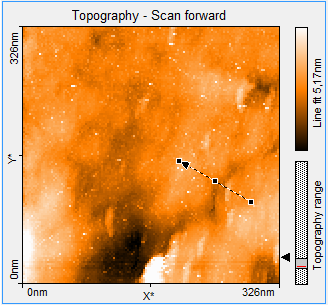
\includegraphics[scale = 0.65]{Kante_5_oberflaeche.png}
\caption{Abschnitt, auf dem die Stufe aufgenommen wurde}
\label{subfig:gold_stufen_a}
\end{subfigure}
\hspace{0.02\textwidth}
\begin{subfigure}[c]{0.49\textwidth}
\centering
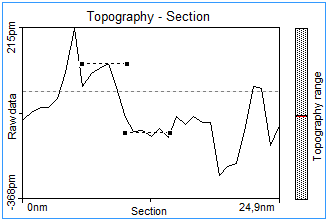
\includegraphics[scale = 0.65]{Kante_5_2d.png}
\caption{Topographischer Verlauf entlang des gew�hlten Weges. Die H�he der Stufe betr�gt 237,8 $\pm$ 11,9 pm}
\label{subfig:gold_stufen_b}
\end{subfigure}
\caption{Beispielhafte Darstellung einer mono atomaren Stufe}
\label{fig:gold_stufen_c}
\end{figure}

Um ein gutes Ergebnis zu erhalten, wurden mehre Messungen gemacht. Da nicht gen�gend einatomige Stufen vorhanden waren, wurden Stufen h�herer Ordnungen hinzugenommen. Dabei wurde die Ordnung der Stufe jeweils gesch�tzt. Die Fehler wurden je nach Rauschen mit 5\% bis 10\% abgesch�tzt. Die gemessenen Werte sind in Tabelle \ref{tab:gold_stufen} zu sehen.


\begin{table}[H]
\centering
\caption{Gemessene Stufen f�r die Bestimmung des Netzebenenabstandes von Goldatomen. Die Fehler wurden dabei mit 5\% bis 10\% abgesch�tzt. n gibt die Ordnung der Stufe an, diese wurden jeweils gesch�tzt}
\label{tab:gold_stufen}
\begin{tabular}{c|c|c}
Stufenh�he/pm & n & Netzebeneabstand/pm \\ \hline
\hline 236 $\pm$ 12 & 1 & 236 $\pm$ 12 \\ 
\hline 236 $\pm$ 12 & 1 & 236 $\pm$ 12 \\ 
\hline 243 $\pm$ 12 & 1 & 243 $\pm$ 12 \\ 
\hline 234 $\pm$ 12 & 1 & 234 $\pm$ 12 \\ 
\hline 238 $\pm$ 12 & 1 & 238 $\pm$ 12 \\ 
\hline 959 $\pm$ 48 & 4 & 239 $\pm$ 12 \\ 
\hline 714 $\pm$ 36 & 3 & 238 $\pm$ 12 \\ 
\hline 935 $\pm$ 47 & 4 & 234 $\pm$ 12 \\
\end{tabular} 
\end{table}

Aus den Messdaten ergibt sich ein Mittelwert von $\bar{d}$=(237$\pm$)4pm dieser Weicht relativ um 0,42\% vom Erwartungswert 236pm ab. Das Ergebnis entspricht einer guten Messung. Es sei jedoch gesagt, dass speziell nach ``guten'' Kanten gesucht wurde, wodurch nicht sichergestellt ist, dass der bestimmte Wert die Gesamtheit der Kanten repr�sentiert. Durch das aussuchen der Kanten wurde jedoch verhindert, dass Kanten, die von Gittersch�den kommen ausgewertet wurden. In Abbildung \ref{fig:gold_defekt} ist ist auf der rechten Seite eventuell ein Gitterdefekt zu sehen.


\begin{figure}[H]
	\centering
  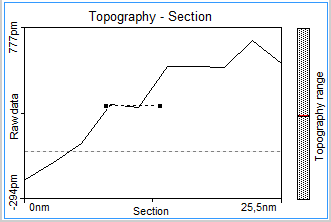
\includegraphics[scale=0.6]{defekt.png}
	\caption{Der Peak an der rechten Seite k�nnte ein Gitterdefekt sein, seine H�he entspricht ca. dem halbem Netzebenenabstand von Gold.}
	\label{fig:gold_defekt}
\end{figure}

\subsection{Unbekannte Probe}
\subsubsection{Rauheit}